\documentclass{article}

\usepackage{latexsym}
\usepackage{bbm}
\usepackage[small,bf]{caption2}
\usepackage{graphics}
\usepackage{epsfig}
\usepackage{amsmath,amssymb,amsthm,amsfonts}
\usepackage{url}
\usepackage{hyperref}
\usepackage{enumerate}
\usepackage[most]{tcolorbox}
\usepackage{xcolor}

\usepackage{tikz}
\usetikzlibrary{shapes.geometric, arrows}

%% Page size
\setlength{\oddsidemargin}{0pt}
\setlength{\evensidemargin}{0pt}
\setlength{\textwidth}{6.5in}
\setlength{\topmargin}{0in}
\setlength{\textheight}{8.5in}

% Footnote commands.
\newcommand{\footnotenonumber}[1]{{\def\thempfn{}\footnotetext{#1}}}
\newcommand{\footnotetight}[1]{\footnote{\renewcommand\baselinestretch{1}\footnotesize #1}}

\newcommand*{\unk}{\texttt{UNK}}

\newtheorem{propo}{Proposition}[section]
\newtheorem{lemma}[propo]{Lemma}
\newtheorem{definition}[propo]{Definition}
\newtheorem{coro}[propo]{Corollary}
\newtheorem{thm}[propo]{Theorem}
\newtheorem{conj}[propo]{Conjecture}
\newtheorem{fact}[propo]{Fact}
\newtheorem{remark}[propo]{Remark}
\newtheorem{claim}[propo]{Claim}

% Create a custom environment
\newenvironment{solution}{\color{blue}}{}

\setlength{\parindent}{0pt}

\begin{document}
\section{N-gram}
\subsection{N-gram Language Modeling \& Perplexity}
\begin{enumerate}[(a)]
  \item Describe how you built your N-gram models. Provide graphs, tables, charts or other summary evidence to support any claims you make.

  \begin{solution}
    Preprocessing of the corpus includes: 
    \begin{enumerate}[1.]
      \item Strip any newline character
      \item Split by white spaces (two or more consecutive white spaces are all removed)
      \item For each sentence, which is split by white spaces to be a list of tokens, 
      the resulting list is appended with a special stop token \texttt{<STOP>}.
    \end{enumerate}
    Generally, the construction of N-gram count map is to count instances of N-gram in the training
    corpus. Specifically, 
    \begin{enumerate}[1.]
      \item Unigram: Count the frequency of each word in the training corpus. In inference time, 
      the probability of a word $s$ becomes $\frac{C_s}{C_{total}}$ where $C_s$ denotes the count 
      of the word $s$ and $C_{total}$ denotes the total number of tokens in the training corpus.
      \item Bigram: Count the frequency of each bigram, which is a pair $(s_{t-1}, s_t)$ in the 
      training corpus. The structure to store these frequencies is a nested dictionary, where
      the outer key refers to $s_{t-1}$ and the inner key refers to $s_t$. i.e. 
      \texttt{cntr[$s_{t-1}$][$s_{t}$]} is the frequency of $s_{t-1}, s_t$ in the training
      corpus. In inference time, given a previous token $s_{t-1}$, the probability for $s_{t}$
      is given as $\frac{C_{s_{t-1}, s_{t}}}{C_{s_{t-1, \ast}}}$ where $C_{s_{t-1}, s_{t}}$ 
      denotes the frequency of the pair $s_{t-1}, s_{t}$ in the training corpus and 
      $C_{s_{t-1, \ast}}$ refers to the total frequency of any pair that starts with $s_{t-1}$.
      Additionally, for any beginning of the sentence word, $s_{t-1}$ is given as the special 
      start token \texttt{<START>}.
      \item Trigram: Count the frequency of each trigram, which is a triplet
      $(s_{t-2}, s_{t-1}, s_{t})$. The structure to store the frequencies is similar to 
      bigram except that it's nested with three layers. The outer key is $s_{t-2}$, the 
      middle layer key is $s_{t-1}$, and the inner key is $s_{t}$. For beginning of the 
      sentence token, $s_{t-2}$ and $s_{t-1}$ would be \texttt{<START>}. For second 
      token of sentence, $s_{t-2}$ would be \texttt{<START>}. In inference time, given 
      previous two tokens $s_{t-2}, s_{t-1}$, the probability for the next token to be 
      $s_{t}$ is $\frac{C_{s_{t-2}, s_{t-1}, s_{t}}}{C_{s_{t-2}, s_{t-1}, \ast}}$ where 
      $C_{s_{t-2}, s_{t-1}, s_{t}}$ refers to the frequency of the triplet $s_{t-2}, s_{t-1},
      s_{t}$ in the training corpus and $C_{s_{t-2}, s_{t-1}, \ast}$ refers to the total 
      frequency of any triplet that starts with $s_{t-2}, s_{t-1}$.
    \end{enumerate}
  \end{solution}
  
  \item Describe how you computed \textit{perplexity} without any smoothing in a detailed equation, in natural language, or with pseudo code.
  
  \begin{solution}
    Now that we have models that could generate probability of next token provided with previous 
    tokens if the model is bigram or trigram. We calculate the perplexity as follows
    \begin{enumerate}[1.]
      \item For sentences in the corpus, calculate the sentence entropy 
      by the sum of the log probability of each token.
      \item Now that we have sentence entropy, we calculate sentence perplexity by 
      $\text{exp}(-\frac{\text{sentence entropy}}{N_{\text{sentence}}})$ where 
      $N_{\text{sentence}}$ is the number of tokens in the sentence including 
      the special \texttt{<STOP>} token. 
      \item Then the perplexity for the corpus can be calculated by averaging each sentence 
      perplexity calculated from previous steps.
    \end{enumerate}
  \end{solution}
  
  \item What's the potential downside of Laplace smoothing? Back up your claim with empirical evidence.
  
  \begin{solution}
    For Laplace smoothing, since we are using $k = 1$, it assumes we've seen the instance of 
    n-gram we are calculating to be one more times than it actually is. This would get less 
    accurate when $n$ gets larger because the number of pair, triplet, or quadruplet unseen 
    is much larger. Assuming seeing those unseen sequence once would lead the modeled distribution
    more inaccurate. As the table in part (d) and part (e), it shows that $k=1$ is blows up 
    the perplexity score for Bigram and Trigram because it's too large and exaggerating 
    the number of unseen instances to be seen. When $k$ gets smaller, the perplexity score 
    for bigram and trigram becomes smaller because it doesn't over making up the number of unseen 
    instances to be seen.
  \end{solution}

  \item Another extension of Laplace smoothing, instead of adding 1 to the count of each token, 
  is to add $k$, where typically $0 < k < 1$. Try different values for $k$, and describe how 
  different $k$ change the perplexity score differently.

  \begin{solution}
    \begin{enumerate}[1.]
      \item \textit{smoothing with $k = 0.5$} perplexity score
      \begin{center}
        \begin{tabular}{| c | c | c |}
          \hline
          & Train & Dev \\ \hline
          Unigram & 1078.84 & 985.18 \\ \hline
          Bigram & 1053.08 & 1419.76 \\ \hline
          Trigram & 4118.46 & 8558.40 \\ \hline
        \end{tabular}
      \end{center}

      \item \textit{smoothing with $k = 0.2$} perplexity score
      \begin{center}
        \begin{tabular}{| c | c | c |}
          \hline
          & Train & Dev \\ \hline
          Unigram & 1079.66 & 985.33 \\ \hline
          Bigram & 631.21 & 1033.93 \\ \hline
          Trigram & 2066.95 & 6798.56 \\ \hline
        \end{tabular}
      \end{center}

      \item \textit{smoothing with $k = 0.01$} perplexity score
      \begin{center}
        \begin{tabular}{| c | c | c |}
          \hline
          & Train & Dev \\ \hline
          Unigram & 1080.33 & 985.54 \\ \hline
          Bigram & 163.90 & 586.45 \\ \hline
          Trigram & 177.89 & 3860.08 \\ \hline
        \end{tabular}
      \end{center}
    \end{enumerate}

    As mentioned in previous part, decreasing $k$ generally decreases the perplexity 
    score for bigram and trigram because it's more accurately modeling those unseen 
    instances compared to the count of other seen instances. It also has more effects on Trigram because the number 
    of combinations of triplets is much more than the number of combinations of a pair (bigram) or the number of single token (unigram).

  \end{solution}
  
  \item Report the \textit{unsmoothed} and \textit{smoothed with Laplace smoothing version} of
  perplexity scores of the unigram, bigram, and trigram language models for your training, 
  development, and test sets. Briefly discuss the experimental results.

  \begin{solution}
    \begin{enumerate}[1.]
      \item \textit{unsmoothed} perplexity score
      \begin{center}
        \begin{tabular}{| c | c | c | c |}
          \hline
          & Train & Dev & Test \\ \hline
          Unigram & 1080.36 & 985.55 & 998.72 \\ \hline
          Bigram & 77.98 & $-\infty$ & $-\infty$ \\ \hline
          Trigram & 8.54 & $-\infty$ & $-\infty$ \\ \hline
        \end{tabular}
      \end{center}

      \item \textit{Laplace smoothing version} perplexity score
      \begin{center}
        \begin{tabular}{| c | c | c | c |}
          \hline
          & Train & Dev & Test \\ \hline
          Unigram & 1078.00 & 985.31 & 998.24 \\ \hline
          Bigram & 1557.07 & 1866.21 & 1864.07 \\ \hline
          Trigram & 6420.99 & 10184.99 & 10160.80 \\ \hline
        \end{tabular}
      \end{center}
    \end{enumerate}

    On the training set perplexity, Trigram reaches the best because it overfits
    the corpus the most.

    For Bigram and Trigram on Dev and Test set, they go to negative infinity 
    because the probability of the unseen instance of sequences (pair or triplet)
    is zero which results in negative infinity when calculating the perplexity.

    With Laplace smoothing, it does tackle the problem of unseen sequences because 
    it assumes seeing everything one more time. However, it seems to be an overkill
    because there are a lot of unseen sequences. Pretending to see every one of them 
    once is inaccurately modeling the distribution. Therefore, the perplexity scores
    of Trigram on Dev and Test become much higher.
  \end{solution}
\end{enumerate}

\subsection{Interpolation}
\begin{enumerate}[(a)]
  \item Your goal is to find reasonably good combinations of 
  $\lambda_1$, $\lambda_2$, $\lambda_3$. 
  Experiment and report perplexity scores on \textit{training} and 
  \textit{development} sets for five sets of values of 
  $\lambda_1$, $\lambda_2$, $\lambda_3$ that you tried, along with short 
  descriptions of the strategies that you used to find better hyperparameters. 
  In addition, report the training and development perplexity for the values 
  $\lambda_1 = 0.1$, $\lambda_2 = 0.3$, $\lambda_3 = 0.6$.

  \begin{solution}
    \begin{center}
      \begin{tabular}{| c | c | c | c | c | c |}
        \hline
        & $\lambda_1$ & $\lambda_2$ & $\lambda_3$ & Train & Dev \\ \hline
        Run 1 & 0.1 & 0.3 & 0.6 & 11.88 & 534.69 \\ \hline
        Run 2 & 0.225 & 0.3 & 0.475 & 14.22 & 415.12 \\ \hline
        Run 3 & 0.35 & 0.3 & 0.35 & 17.81 & 369.72 \\ \hline
        Run 4 & 0.475 & 0.3 & 0.225 & 24.16 & \textbf{351.08} \\ \hline
        Run 5 & 0.6 & 0.3 & 0.1 & 39.34 & 352.86 \\ \hline
        Run 6 & 0.2 & 0.5 & 0.3 & 18.04 & 377.68 \\ \hline
      \end{tabular}
    \end{center}

    The strategies for hyperparameters search is to first fix $\lambda_2$ and 
    increase/decrease $\lambda_1$/$\lambda_2$ respectively because Bigram lies 
    in between Trigram and Unigram. After five runs, we try to increase $\lambda_2$
    for another run and let $\lambda_1$ and $\lambda_3$ to be roughly equal to observe 
    the effect of increasing $\lambda_2$. 

    From Run 1 to Run 5, as we increase the weight on Unigram, it's normal to observe 
    that the training perplexity increases because Bigram and Trigram are better at 
    fitting the training set. We also see that from Run 1 to Run 4, the dev perplexity 
    decreases as weighing more on Unigram helps with generalization and prevents from 
    Trigram's overfitting. Finally, Run 5 has a higher dev perplexity because it seems 
    to weigh Unigram too much. As for Run 6, compared with Run 3 with similar training 
    perplexity, it doesn't seem to generalize better than Run 3 that weighs Bigram less.
  \end{solution}
    
  \item Putting it all together, report perplexity on the \textit{test} set, 
  using the \textit{best} combination of hyperparameters that you chose from 
  the development set. Specify those hyperparameters.

  \begin{solution}
    The best hyperparameters come from Run 4. The test perplexity is \textbf{354.35}.
  \end{solution}
    
  \item If you use half of the training data, would it increase or decrease the 
  perplexity of previously unseen data? Why? Provide empirical experimental evidence 
  to support your claims.

  \begin{solution}
    We use the best hyperparameters for interpolation and evaluate it on dev set and 
    test set while training it on half of the training set. The resulting dev perplexity 
    is 323.57 and test perplexity is 323.57. This is a decrease in perplexity. We hypothesize
    that it's because using half of the training set can assume lots of \unk in the training 
    corpus, which leads to less surprised model when seeing \unk in the evaluation set.
  \end{solution}
    
  \item If you convert all tokens that appeared less than five times to \unk 
  (a special symbol for out-of-vocabulary tokens), would it increase or decrease 
  the perplexity on the previously unseen data compared to an approach that converts 
  only those words that appeared just once to \unk? Why? Provide empirical evidence 
  to support your claims.

  \begin{solution}
    When converting all tokens that appeared less than five times to \unk , we observe 
    that the dev set perplexity drops to 290.18 and the test set perplexity drops to 
    293.07 with the best hyperparameters combination from previous part. On the other 
    hands, when we convert words that appeared just once to \unk , the dev set perplexity 
    increases to 405.52 and the test set perplexity increases to 405.38.

    We hypothesize that the evaluation set has more unseen data than using 3 as the threshold to model 
    the \unk probability in training set. Increasing the threshold to 5 results in a better perplexity 
    because it'll increase the probability of \unk modeled in training set and thus better describe 
    the probability of unseen data in the evaluation set. On the contrary, decreasing the threshold
    would increase the perplexity on the same evaluation sets because the modeled \unk probability 
    underestimates the probability of unseen data in the evaluation set.

  \end{solution}
\end{enumerate}

\newpage
\section{BPE}
\begin{enumerate}[(a)]
  \item Please produce a scatterplot showing points (x,y), each corresponding to an 
  iteration of the algorithm, with x the current size of the type vocabulary 
  (including the base vocabulary), and y the length of the training corpus (in tokens)
  under that vocabulary's types. How many types do you end up with? What is the 
  length of the training data under your final type vocabulary?

  \begin{solution}
    \begin{center}
      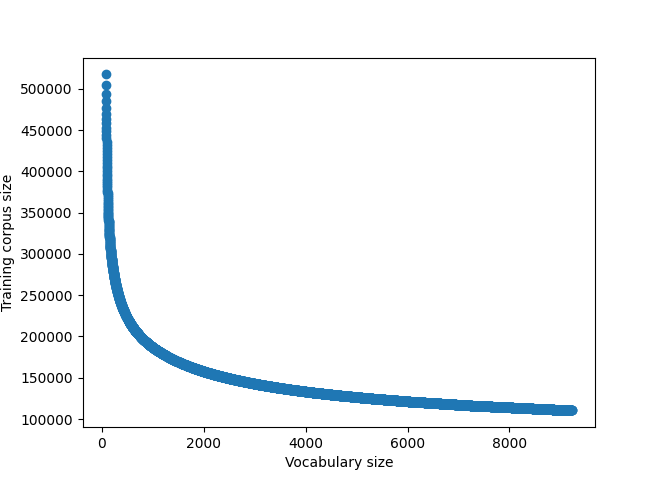
\includegraphics[scale=0.6]{Figure_1.png}
    \end{center}

    \begin{enumerate}[1.]
      \item Length of vocabularies: 9219
      \item Length of training corpus: 110433
    \end{enumerate}
  \end{solution}

  \item Another way of overcoming the rare word issue is to encode text as a 
  sequence of characters. Discuss the advantages and potential issues of character-level
  encoding compared to BPE.

  \begin{solution}
    \begin{enumerate}[]
      \item \textbf{Advantages}: Using character-level encoding can remove any unseen token risk 
      if we include enough ASCII characters. This prevents from extra headache and hyperparameters
      of making \unk in the training corpus.
      \item \textbf{Disadvantages}: Character-level encoding would be insanely memory inefficient because
      there is no merging and every token is stored as a list of individual tokens. In addition,
      this tokenization doesn't encode any more information beyond the character, which means 
      the semantics can hardly be encoded within the token. 
    \end{enumerate}
  \end{solution}
  
  \item Applying your tokenizer on the last 1000 lines of the data, how many tokens 
  do you end up with? Do you encounter issues with words that didn't appear in the 
  training set? More generally, when would you expect your tokenizer to fail when 
  applying to an unseen text.

  \begin{solution}
    \begin{enumerate}[1.]
      \item Number of tokens in last 1000 lines: 30025
      \item Didn't encounter unseen tokens in the last 1000 lines. The tokenizer
      will fail to apply to an unseen text if there exists individual character 
      that doesn't appear in the training set because we start the tokenization 
      with a vocab set of all characters in the training corpus which does not 
      necessarily guarantee all individual characters in English or punctuation.
    \end{enumerate}
  \end{solution}
\end{enumerate}

\newpage
\section{Wordpiece}
\begin{enumerate}
  \item Please produce a scatterplot showing points (x,y), each corresponding to 
  an iteration of the algorithm, with x the current size of the type vocabulary 
  (including the base vocabulary), and y the length of the training corpus (in tokens) 
  under that vocabulary's types. How many types do you end up with? What is the 
  length of the training data under your final type vocabulary?

  \begin{solution}
    \begin{center}
      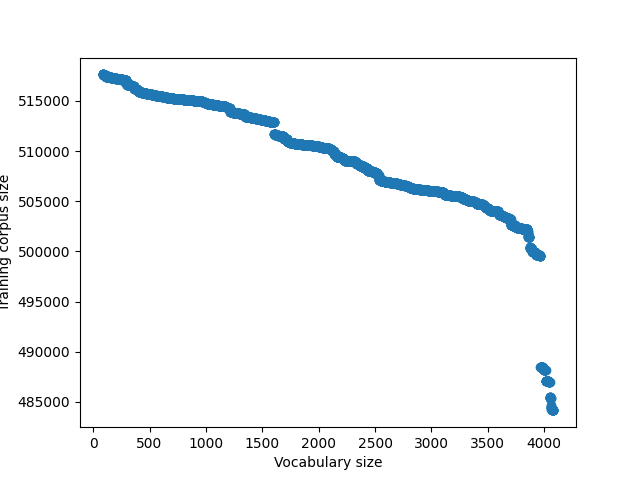
\includegraphics[scale=0.6]{Figure_2.png}
    \end{center}

    \begin{enumerate}[1.]
      \item Length of vocabularies: 4083
      \item Length of training corpus: 484152
    \end{enumerate}
  \end{solution}

  \item Applying your tokenizer on the last 1000 lines of the data, report the 
  length of the tokenized data. Also, include the tokenized sequences for the 
  following two sentences: 

  \begin{enumerate}
      \item \textit{``Analysts were expecting the opposite, a deepening of the deficit.''}
      \item \textit{``Five minutes later, a second person arrived, aged around thirty, with knife wounds.''}
  \end{enumerate}

  \begin{solution}
    \begin{enumerate}[1.]
      \item Length of tokenized evaluation data (last 1000 lines): 115490
      \item The tokenized sequence for the two sentences
      
      \texttt{['A', 'n', 'a', 'l', 'y', 's', 't', 's', '<B>', 'w', 'e', 'r', 'e', '<B>', 'exp', 'e', 'c', 't', 'i', 'n', 'g', '<B>', 'th', 'e', '<B>', 'o', 'p', 'p', 'o', 's', 'i', 't', 'e', ',', '<B>', 'a', '<B>', 'd', 'e', 'e', 'p', 'e', 'n', 'i', 'n', 'g', '<B>', 'o', 'f', '<B>', 'th', 'e', '<B>', 'd', 'e', 'f', 'i', 'c', 'i', 't', '.']}

      \texttt{['F', 'i', 'v', 'e', '<B>', 'm', 'i', 'n', 'u', 't', 'e', 's', '<B>', 'l', 'a', 't', 'e', 'r', ',', '<B>', 'a', '<B>', 's', 'e', 'c', 'o', 'n', 'd', '<B>', 'p', 'e', 'r', 's', 'o', 'n', '<B>', 'a', 'r', 'r', 'i', 'v', 'e', 'd', ',', '<B>', 'a', 'g', 'e', 'd', '<B>', 'a', 'r', 'o', 'u', 'n', 'd', '<B>', 'th', 'i', 'r', 't', 'y', ',', '<B>', 'w', 'i', 'th', '<B>', 'k', 'n', 'i', 'f', 'e', '<B>', 'w', 'o', 'u', 'n', 'd', 's', '.']}
    \end{enumerate}
  \end{solution}

  \item In terms of efficiency and performance, what's the advantages and disadvantages 
  of WordPiece compared with BPE? There is no single correct answer here, just 
  provide your thoughts and rationales, supported by empirical evidences.

  \begin{solution}
    \begin{enumerate}
      \item Advantages: WordPiece seeks to merge those with highest normalized frequency
      which results in tokens like links or email address because of the frequencies of 
      individual tokens on the denominator. This helps with tokenizing those types of 
      words or tokens compared to BPE because those links and email address would remain 
      intact to retain its meaning. This is empirically supported by examining the top 10 
      longest tokens in the rules learned in WordPiece.

      \item Disadvantages: WordPiece is not as efficient as BPE because it requires counting 
      the frequencies of each token to calculate the normalized pair frequency to merge.
      In addition, the number of seconds taken to run BPE is roughly the same as WordPiece
      but WordPiece is only able to run for 4000 iterations versus BPE is able to run for 
      about 9000 iterations. This is empirically supported by timing the BPE and WordPiece which 
      both result in around 260 seconds (257.14s for WordPiece / 275.65s for BPE)
    \end{enumerate}
  \end{solution}

\end{enumerate}

\end{document}